\documentclass[tikz,10pt,border=2mm]{standalone}
\usepackage{mathpazo,structmech,siunitx}
\usetikzlibrary{calc}
\begin{document}
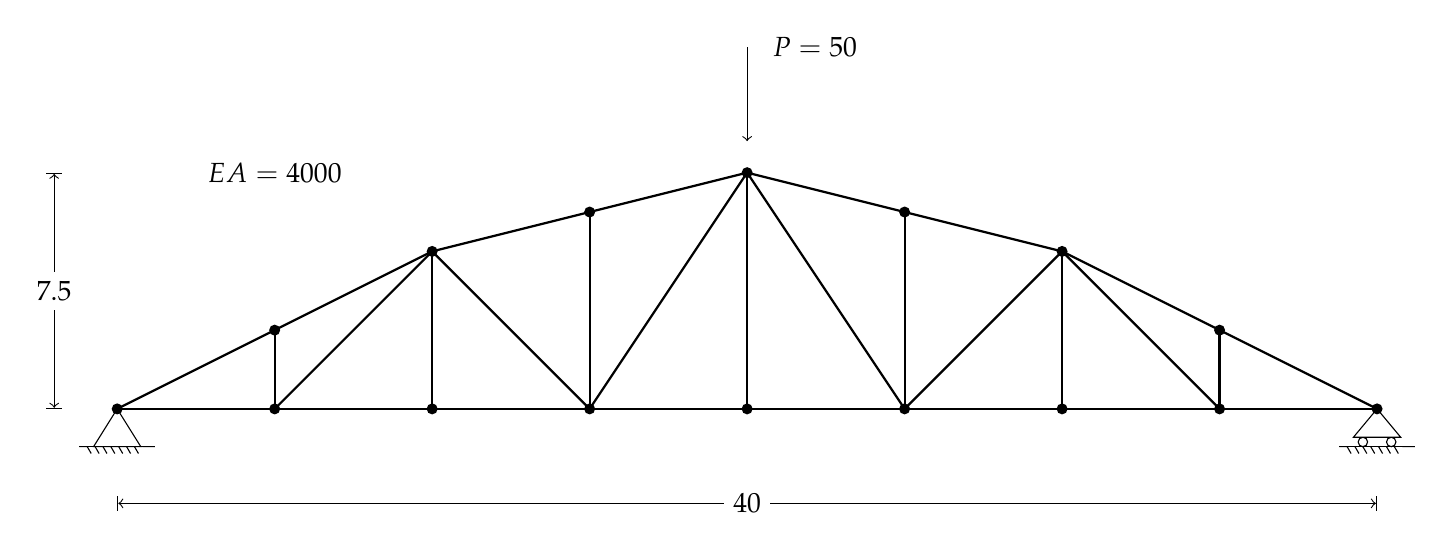
\begin{tikzpicture}[scale=.4]
\setstructmech{linewidth=.4pt}
\coordinate(N14)at(0,0);
\coordinate(N11)at(5,0);
\coordinate(N12)at(5,2.5);
\coordinate(N10)at(10,0);
\coordinate(N13)at(10,5);
\coordinate(N1)at(15,0);
\coordinate(N2)at(15,6.25);
\coordinate(N15)at(20,0);
\coordinate(N3)at(20,7.5);
\coordinate(N4)at(25,0);
\coordinate(N9)at(25,6.25);
\coordinate(N5)at(30,0);
\coordinate(N8)at(30,5);
\coordinate(N6)at(35,0);
\coordinate(N7)at(35,2.5);
\coordinate(N16)at(40,0);
\begin{scope}[every node/.style={inner sep=0,circle,fill=black,minimum size=1.4mm}]
\node at(N1){};
\node at(N2){};
\node at(N3){};
\node at(N4){};
\node at(N5){};
\node at(N6){};
\node at(N7){};
\node at(N8){};
\node at(N9){};
\node at(N10){};
\node at(N11){};
\node at(N12){};
\node at(N13){};
\node at(N14){};
\node at(N15){};
\node at(N16){};
\end{scope}
\begin{scope}[line width=.8pt]
\draw(N1)--(N2);
\draw(N3)--(N2);
\draw(N4)--(N3);
\draw(N5)--(N4);
\draw(N6)--(N5);
\draw(N6)--(N7);
\draw(N8)--(N7);
\draw(N9)--(N8);
\draw(N4)--(N9);
\draw(N1)--(N3);
\draw(N10)--(N1);
\draw(N11)--(N10);
\draw(N11)--(N12);
\draw(N13)--(N12);
\draw(N13)--(N11);
\draw(N14)--(N11);
\draw(N12)--(N14);
\draw(N2)--(N13);
\draw(N15)--(N3);
\draw(N4)--(N15);
\draw(N8)--(N4);
\draw(N8)--(N5);
\draw(N8)--(N6);
\draw(N7)--(N16);
\draw(N3)--(N9);
\draw(N1)--(N15);
\draw(N13)--(N1);
\draw(N13)--(N10);
\draw(N16)--(N6);
\end{scope}
\draw[<-]($(N3)+(0,1)$)--++(0,3)node[right=2mm]{$P=50$};
\HingeSupport{N14}{3};
\RollerSupport{N16}{3};
\node at(5,7.5){$EA=4000$};
\draw[|<->|](0,-3)--++(40,0)node[midway,fill=white]{$40$};
\draw[|<->|](-2,0)--++(0,7.5)node[midway,fill=white]{$7.5$};
\end{tikzpicture}
\end{document}